
\chapter{Addressing Weakly-coupled Carbon Spins}

The electronic-spin of the NV-center does not live in a vacuum but in an environment full of nuclear spins.
To some of these spins the NV-center couples strongly, these spins can be controlled and can serve as qubits.
To others it couples weakly these spins are a source of decoherence and cannot be controlled directly.

In this chapter I will first explain what strong and weakly coupled spins are, how this relates to coherence and how coherence can be extended trough dynamical decoupling.
In the second part of this chapter I will explain how dynamical dynamical decoupling can be used to identify and control some of these weakly coupled spins, transforming them from a source of decoherence to a resource for qubits.

\begin{figure}[htbp]
\centering
    \begin{tikzpicture}
        \node[anchor=south west,inner sep=0] at (0,0) {\includegraphics[scale = 0.5]{Img/coupling_regimes.eps}};
        \node[font=\tiny] at (5,4) {$A \approx \frac{\sqrt{\ln{2}}}{\pi T_{2\mathrm{C}}^*}$};
        \node[font=\tiny] at (4,3.1) {$A\approx \frac{\sqrt{\ln{2}}}{\pi T_{2e}^*}$};
        \node[font=\small] at (3.8,1.9) {$\mathbb{I}$};
        \node[font=\small] at (4.75,1.2) {$\mathbb{II}$};
        \node[font=\small] at (5.6,0.5) {$\mathbb{III}$};
        %Help grid for drawing
        % \draw[help lines,xstep=1,ystep=1] (0,0) grid (7,5);
        % \foreach \x in {0,1,...,7} { \node [anchor=north] at (\x,0) {\x}; }
        % \foreach \y in {0,1,...,5} { \node [anchor=east] at (0,\y) {\y}; }
    \end{tikzpicture}
    \caption{ Schematic representation of different coupling regimes. In the strong coupling regime (region $\mathbb{I}$) carbon-spins are coupled to the NV-center stronger than the coupling of the NV-center to the spin-bath. These carbons can be addressed directly. In the weak coupling regime (region $\mathbb{II}$) carbon-spins are coupled more strongly to the NV-center than to the spin-bath but not strong enough to be addressed directly. In the very-weak coupling regime (region $\mathbb{III}$) the coupling to the spin-bath is stronger than the coupling to the NV-center. These spins cannot be addressed.}
    \label{fig:coupling regimes}
\end{figure}

\section{Coupling to the Environment}


\subsection{Coupling regimes}
When addressing a spin qubit we usually drive transitions between energy levels.
When the electronic-spin couples to a nuclear-spin these energy levels are shifted depending on the state of the nucleus.
In this way each spin has an individual back-action on the electronic-spin.

Most of these spins only shift the spin by a tiny amount making it hard to distinguish them from each other.
Because the states of these spins fluctuate the transitions of the NV-center are continuously shifting around, effectively causing a broadening of the transitions.
We call these very-weakly-coupled spins the spin-bath.

If the coupling between a spin and the NV-center is strong enough it is possible to resolve and address its transitions.
Transitions between energy levels can be resolved if the difference between them is larger than the width of transition.


The width of the transitions is related to the rate at which the transitions shift out of resonance.
The time before a transition shifts out of resonance, or a signal decoheres, is usually expressed by $T_2^*$ and is measured by a Ramsey experiment, see \cref{fig:Ramsey_gijs}.

\begin{figure}[htbp]
    \centering
    \includegraphics{Img/Ramsey_Gijs.pdf}
    \caption{In a Ramsey experiment a qubit in initialized along the z-axis before being subjected to a $\pi/2$-pulse that moves it into the xy plane of the Bloch-sphere. It freely evolves for a time $\tau$ before being subjected to a final $\pi/2$ pulse and read out along the z-direction.
The final pulse will rotate the spin towards the poles depending on the phase picked up during free evolution. This manifests itself as an oscillation. This oscillation will slowly decay because the final pulse will be more out of resonance with the transition the longer the free evolution time. Figure from \citep{Lange2012Quantum}.}
    \label{fig:Ramsey_gijs}
\end{figure}

The decay of the amplitude $K$ in an electron Ramsey experiment is given by \cref{eq:Ramsey_decay}.
\begin{equation}
    K(t) = e^{-(\tfrac{\tau}{T_{2e}^*})^2}
    \label{eq:Ramsey_decay}
\end{equation}
We define $T_{2e}^*$ as the $1/e$ value of the Gaussian decay. The dark Electron-Spin-Resonance (ESR)\footnote{See \cref{fig:HF_split_levels} for an example of a dark ESR.} frequency spectrum for negligible power broadening is given by the Fourier transform of \cref{eq:Ramsey_decay}. Where $\omega = 2\pi \cdot f$\footnote{For clarity the factor of $2\pi$ is stated explicitly throughout this thesis to distinguish real and angular frequency. }.
\begin{equation}
    \mathcal{F} \{ K(\tau) \} =  T_2^* \sqrt{\pi} e^{-\tfrac{(2\pi \cdot f) ^2 \cdot T_{2e}^{*2}}{ 4}}
\end{equation}
Two identical Gaussians can be readily resolved if the separation between their maxima is larger than their full-width-half-maximum (FWHM).
The FWHM of the dark ESR is given by \cref{eq:FWHM}.
\begin{equation}
    2\pi \cdot \mathrm{FWHM} = 2\pi \cdot \frac{2\sqrt{\ln{2}}}{\pi T_{2e}^*}
    \label{eq:FWHM}
\end{equation}

We define a spin to be strongly coupled when it is possible to readily resolve its transition.
For a carbon-spin that is when twice the interaction strength $A$ [NOTE: $|A|$? A par? shift due to A? ] is larger than the FWHM of the transition:
\begin{equation}
     2\pi \cdot A> 2\pi \cdot \frac{\sqrt{\ln{2}}}{\pi T_{2e}^*}
     \label{eq:def_strongly_coupled}
 \end{equation}

NV-centers have a typical electron $T_{2e}^* \approx 2\mu \mathrm{s}$\footnote{At a natural concentration of $1.1 \%$ carbon-13.} that depends on the exact configuration of the spin-environment. Increasing the carbon-13 concentration generally reduces $T_{2e}^*$.
For a typical NV-center this means that the coupling between the carbon and the NV-center must be larger than $2\pi\cdot$130kHz for the carbon to be directly addressable.


\subsection{The Hyperfine Interaction}
The coupling between the NV-centers electronic spin and a nuclear-spin is given by the hyperfine-interaction. The hyperfine-interaction is a spin dependent interaction that is not present for spin-0 particles such as carbon-12.

For nuclear spins the Hamiltonian depends on the electronic spin-state of the NV-center.
For a magnetic field ($B_\mathrm{z}$) in the z-direction the Hamiltonian is given by \cref{eq:nuclear_hamiltonian_0} when the electronic-spin is in the $m_s = 0$ state, and by \cref{eq:nuclear_hamiltonian_1} when in the $m_s = +1$ state\citep{Taminiau2014Universal}. Where $\gamma_n$ is the gyro-magnetic ratio of the nucleus.
 \begin{equation}
 \label{eq:nuclear_hamiltonian_0}
H_0= \gamma_{n} B_\mathrm{z} I_\mathrm{z}
\end{equation}
\begin{equation}
 \label{eq:nuclear_hamiltonian_1}
    H_1 = \gamma_{n} B_\mathrm{z} I_\mathrm{z} +H_{\mathrm{HF}}
\end{equation}

The Larmor frequency for a nucleus is given by  \cref{eq:nuclear_larmor}.
\begin{equation}
\label{eq:nuclear_larmor}
\bm{\omega_L} = \gamma_{n}B_\mathrm{z} \cdot\bm{\hat{\mathrm{z}}}
\end{equation}

The hyperfine ($H_{\mathrm{HF}}$) term consists of a contact term and a dipole term.
The contact term results from an overlap between the electronic- and nuclear- wave-functions making it negligible for all but the nuclear-spins closest to the NV-center.

\begin{figure}[htbp]
\centering
    \begin{tikzpicture}
        \node[anchor=south west,inner sep=0] at (0,0) {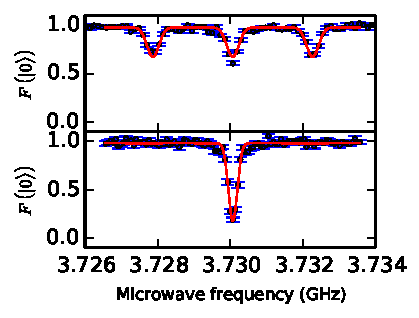
\includegraphics{Img/DarkESR_2.pdf}};
        \node (A) at (2.6,4.4) {};
        \node (B) at (3.92,4.4) { };
        \node (C) at (5.3,4.4) { };
        \draw[latex-latex, font=\small] (A) -- node[label =270: $A_\mathrm{N}$] {} (B);
        \draw[latex-latex, font=\small] (B) -- node[label =270: $A_\mathrm{N}$] {} (C);
    \end{tikzpicture}
    \caption{dark Electron Spin Resonance (ESR) for uninitialized (top) and initialized nitrogen spin (bottom) of the $m_s =0 \rightarrow m_s = +1$ transition. In a dark ESR the spin is prepared in $\ket{0}$, a microwave pulse is applied and then the $\ket{0}$ state is read-out again. This is done for a range of frequencies. When the microwave is on resonance with a transition the spin will be rotated and a dip will be visible in the signal. In the top figure the transition is split due to the interaction with the nearby nitrogen atom. In the lower figure the nitrogen state is initialized and the splitting disappears.}
    \label{fig:HF_split_levels}
\end{figure}

\subsection{Strongly-coupled spins}
An example of a strongly coupled spin is the NV-nitrogen spin.
The strength of the coupling between the nitrogen and the electronic spin is $A_\mathrm{N} = 2\pi \cdot 2.186\quad \mathrm{MHz} $\citep{Bernien2014Control} and it acts along the NV-axis.
\Cref{fig:HF_split_levels} clearly shows the $m_s =0 \rightarrow m_s=+1$ transitions being split due to hyperfine-coupling to the nitrogen.
This splitting can be used to control the nitrogen.
By first initializing in the $m_s =+1$-state and then applying a slow pulse that turns only one of the three nitrogen spin-states back to $m_s=0$ and reading out the nitrogen-spin can be initialized. By only continuing on a positive outcome the spin is initialized in the state that was rotated back to $m_s =0$. We call this measurement-based-initialization (MBI).
The lower panel of \cref{fig:HF_split_levels} shows a dark Electron-Spin-Resonance (ESR) after nitrogen-MBI.

In a similar way strongly-coupled carbon-13 atoms can be controlled\citep{Robledo2011HighFidelity}.
For most strongly-coupled carbons the contact term in the hyperfine is not negligible.
For these carbons hyperfine couplings have been measured\citep{Smeltzer201113} and calculated\citep{Gali2008Ab,Gali2009Identification}.

\subsection{Weakly-coupled carbon spins}
For carbons where the contact term is negligible the hyperfine-term is equal to the dipole term and is given by \cref{eq:dipole_component_of_hyperfine}\citep{Lange2012Quantum}.
With $n_\mathrm{HF}$ is a unit vector pointing from the NV-center to the nucleus and $r$ the distance between them.
$\mathbf{S}$ and $\mathbf{I}$are the spin operators for the NV-spin and the nucleus, $\gamma_e $ the gyromagnetic ratio of the electron, $\gamma_n$ the gyromagnetic ratio of the nucleus, and $\mu_0$ the magnetic permeability.
For weakly-coupled carbons the contact-term of the hyperfine is generally\footnote{Only under exceptionally high carbon-13 concentrations is $T_{2e}^*$ short enough for close by carbon-13 atoms to fall under the definition of weakly coupled. } negligible.

\begin{equation}
\label{eq:dipole_component_of_hyperfine}
H_{\mathrm{dip}} = \frac{\mu_0 \gamma_e \gamma_{\mathrm{C}} \hbar^2 }{4 \pi r^3} [ \bm{S \cdot I} - 3 (\bm S \cdot \hat{n_{\mathrm{hf}}})(\bm I \cdot \hat{n_{\mathrm{hf}}})]
\end{equation}

From \cref{eq:dipole_component_of_hyperfine}  the parallel and orthogonal components of the Hyperfine interaction, with respect to the NV-axis along the z-direction, can be derived to be:
 \begin{align}
A_\parallel= - \frac{\mu_0 \gamma_e \gamma_{\mathrm{C}} \hbar^2 }{4 \pi r^3} \left(3\cdot \frac{z^2}{r^2}-1\right)\\
 A_\perp =  -\frac{\mu_0 \gamma_e \gamma_{\mathrm{C}} \hbar^2 }{4 \pi r^3}\left( 3\cdot\frac{\sqrt{x^2+y^2}\cdot z}{r^2}\right)
\end{align}
Where $H_{\mathrm{HF}} = A_\parallel I_\mathrm{z} + A_\perp I_x $.

At first sight it seems impossible to control weakly coupled spins as their transitions are obscured by the spin-bath.
It is however possible to increase the coherence time of the electron, stabilizing the transitions, allowing more spins to be resolved.

\subsection{Extending electron coherence}
In a spin-echo experiment a Ramsey experiment is performed with a small difference. An additional $\pi$ pulse is applied in the middle of the experiment exactly between the $\pi/2$ pulses. This pulse effectively turns the nuclear-spin environment upside-down halfway trough the experiment, making the qausi-static-part of the dephasing during the first and the second part of the free evolution cancel each other out, substantially increasing coherence on short-timescales ($\tau \ll T_2 $)
\footnote{ $T_2$ is a measure for decoherence. It is similar to $T_2^*$ but does not include variations between experiments. $T_2$ is defined as the $1/e$ time of the decay of a spin-echo experiment.}.
On longer timescales the difference between the initial part of the evolution and the final part of the evolution becomes larger making the initial and final part no longer cancel each other out.

A natural way of extending the short timescale behavior of the spin-echo to longer timescales is by applying more $\pi$-pulses. This procedure known as dynamical-decoupling can dramatically improve coherence times by decoupling the central-spin from the environment\citep{Lange2010Universal}.

Although dynamical-decoupling improves the coherence of the central spin by decoupling from the environment, the central spin is also decoupled from other spins preventing direct two-qubit gates. It was demonstrated by \citet{Sar2012DecoherenceProtected} how to incorporate dynamical decoupling in a universal gate design by implementing Grover's algorithm.
Using this technique \citet{Taminiau2012Detection} used the extended coherence to detect and control weakly-coupled carbon spins, before implementing three-qubit quantum-error-correction (QEC) \citep{Taminiau2014Universal}.

As these experiments where performed with NV-centers at Room temperature they lack the option to do single-shot readout required to act on a measurement outcome\footnote{@Tim, I think this can be worded more concisely. Do you have any ideas?}. An essential feature for the parity measurements that form the basis of measurement-based QEC and surface codes.

\subsection{Dynamical decoupling spectroscopy}
As we cannot perform an ESR experiment while decoupling a different technique must be used to resolve and address additional spins.
In order to resolve additional spins we perform a dynamical decoupling spectroscopy, resulting in a fingerprint of the nuclear-spin environment\citep{Taminiau2012Detection}.

In a dynamical decoupling spectroscopy experiment the electron is prepared in the $|X\rangle = |0\rangle +|1\rangle$ state. It is subjected to a decoupling sequence consisting of N/2 blocks of the form {$\tau - \pi -2\tau-\pi-\tau$}, and concluded by measuring $\langle X\rangle $. The fingerprint is the result of many repetitions for a range of inter-pulse delays $2\tau$. $\pi$ is a $\pi$-pulse.

Part of a dynamical decoupling spectroscopy can be seen in \cref{fig:FP}. The spectroscopy was performed for N = 8, 16, 32 and 64 pulses. For N = 8, 16 and 32 pulses this was done between $\tau = 2 \mu \mathrm{s}$  and $72 \mu \mathrm{s}$ and for N = 64 this was done up to $\tau = 52 \mu \mathrm{s}$. A reference to the full spectroscopy can be found in \cref{chap:Fingerprint_data_appendix}.

\begin{figure}[htbp]

    \begin{subfigure}[t]{\textwidth}\centering
        \begin{tikzpicture}
            \node[anchor=south west,inner sep=0] at (0,0) {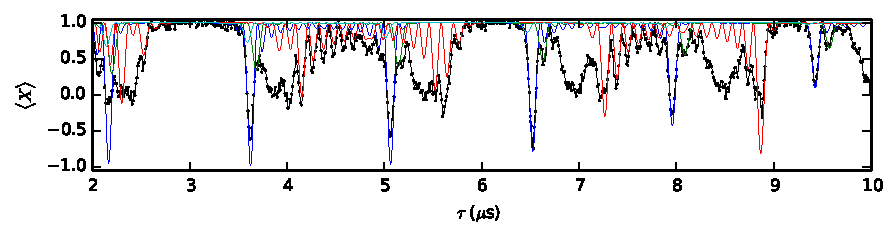
\includegraphics{Img/fingerprint16.pdf}};
            \node[font=\small, text = blue] at (4.05,1.7)  {1};
            \node[font=\small, text = green] at (9.3,2.9) {2};
            \node[font=\small, text = red] at (5.3,2.5) {3};
            \node[font=\small, text = cyan] at (4.0,3.35) {4};
            % \draw[help lines,xstep=1,ystep=1] (0,0) grid (10,3);
            % \foreach \x in {1,2,...,10} { \node [anchor=north] at (\x,0) {\x}; }
            % \foreach \y in {1,2,...,3} { \node [anchor=east] at (0,\y) {\y}; }
        \end{tikzpicture}
        \caption{Fingerprint for N=16 pulses. }
        \label{fig:FP16}

    \end{subfigure}

    \begin{subfigure}[t]{\textwidth}\centering

    \begin{tikzpicture}
        \node[anchor=south west,inner sep=0] at (0,0) {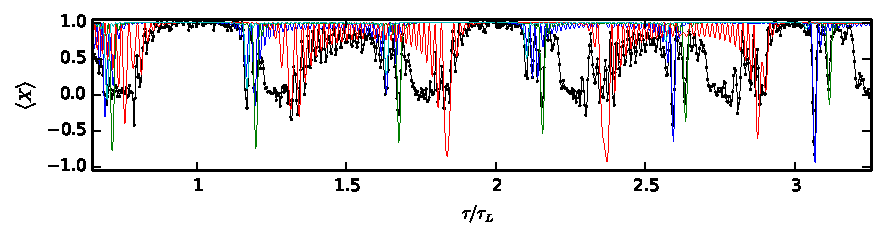
\includegraphics{Img/fingerprint32.pdf}};
        \node[font=\small, text = blue] at (11.2,1.9) {1};
        \node[font=\small, text = blue] at (4.0,2.8)  {1};
        \node[font=\small, text = green] at (6.6,1.8) {2};
        \node[font=\small, text = red] at (7.4,1.8) {3};
        \node[font=\small, text = cyan] at (4.05,2.5) {4};
        % \draw[help lines,xstep=1,ystep=1] (0,0) grid (10,3);
        % \foreach \x in {1,2,...,10} { \node [anchor=north] at (\x,0) {\x}; }
        % \foreach \y in {1,2,...,3} { \node [anchor=east] at (0,\y) {\y}; }
    \end{tikzpicture}
        % \centering
        % 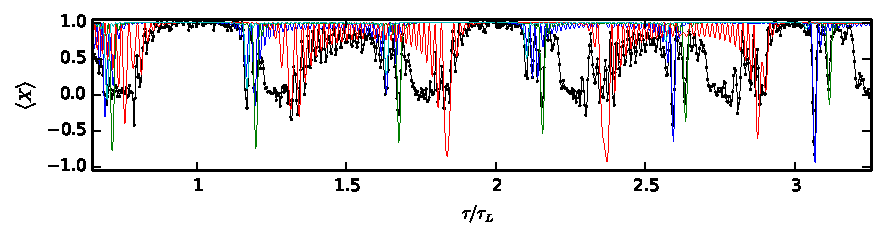
\includegraphics{Img/fingerprint32.pdf}
        \caption{Fingerprint for N =32 pulses. }
        \label{fig:FP32}
    \end{subfigure}
    \caption{Part of a fingerprint resulting from a dynamical-decoupling-spectroscopy experiment performed at 304.12G. A reference to the full spectroscopy can be found in \cref{chap:Fingerprint_data_appendix}.  Colored lines represent computed responses of carbon spins. Responses were calculated using \cref{eq:contrast_single_carbon_spin} with hyperfine parameters from \cref{tbl:HF_par}. }
    \label{fig:FP}
\end{figure}

\section{Addressing Weakly-coupled Carbons through Dynamical Decoupling}
\label{sec:controllingacarbonthroughdynamicaldecoupling}

In order to understand how the features in the fingerprint from \cref{fig:FP} relate to the different spins and how this knowledge can be used to control these carbons it is necessary to understand what dynamical decoupling does to these atoms.

\subsection{The effect of dynamical decoupling}

\begin{figure}[htbp]
\centering
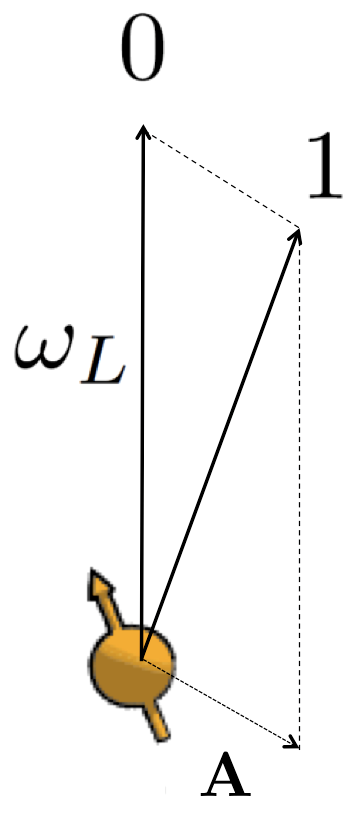
\includegraphics[keepaspectratio,width=0.15\textwidth]{./img/QuantizationAxis.png}
\caption{Flipping the electron spin from the  $m_s=0$ to the $m_s= +1$ state changes the quantization axis of nuclear spins. For  $m_s=0$ all nuclear spins precess about $\bm{\omega_L}$. For  $m_s=+1$ each spin precesses about a distinct axis $\bm{\tilde{\omega}}=\bm{\omega_L} +\bm{A}$.}
\label{fig:quantax}
\end{figure}

When the electron is in the $m_s=0$ state each nuclear spin precesses about $\bm{\omega_L}$ with the Larmor frequency. When the electron is in the $m_s=+1$ state nuclear spins precess about a distinct axis $\bm{\tilde{\omega}}=\bm{\omega_L} +\bm{A}$ \citep{Taminiau2012Detection}. The hyperfine interaction $\bm{A}$ depends on the position of that particular nuclear spin relative to the NV- center.

When applying a decoupling sequence with N\slash 2 decoupling units of the form {$\tau - \pi -2\tau-\pi-\tau$}, the nuclear spin alternately rotates around the  $\bm\omega_L$ and the $\bm{\tilde{\omega}}$ axis.
The net result of one such decoupling sequence is a rotation around an axis $\bm{\hat{\mathrm{n_i}}}$ by an angle $\phi$.
Where $\bm{\hat{\mathrm{n_i}}}$ depends on the initial state of the electron: $\bm{\hat{\mathrm{n_0}}}$ when the electron starts in $m_s = 0$ and $\bm{\hat{\mathrm{n_1}}}$ when the electron starts in $m_s = +1$~\citep{Taminiau2012Detection}.

\begin{figure}[htbp]
    \begin{subfigure}[t]{0.49\textwidth}\centering
        \centering
        \includegraphics{Img/unCond_rot_taminiau.pdf}
        \caption{Unconditional rotation.}
        \label{fig:uncond_rot}
    \end{subfigure}
    \begin{subfigure}[t]{0.49\textwidth}\centering
        \centering
        \includegraphics{Img/Cond_rot_taminiau.pdf}
        \caption{Conditional rotation.}
        \label{fig:cond_rot}
    \end{subfigure}
    \caption{\Cref{fig:uncond_rot} When the net rotation axes $\bm{\hat{\mathrm{n_0}}}$ and $\bm{\hat{\mathrm{n_1}}}$ point in the same direction the carbon experiences an unconditional rotation and cannot be controlled. \Cref{fig:cond_rot} When the net rotation axes $\bm{\hat{\mathrm{n_0}}}$ and $\bm{\hat{\mathrm{n_1}}}$ are anti-parallel the carbon experiences a conditional rotation, either around +x or -x, and can be controlled.}
    \label{fig:conditional_and_unconditional_rotation}
\end{figure}


To understand how a carbon-13 atom can be controlled it is useful to consider three situations. In the first situation the $\bm{\omega_L}$ and $\bm{A}$ point in the same direction. In the second situation $\bm{\omega_L}$ and $\bm{A_\perp}$ are of comparable magnitude, resulting in a large angle between the quantization axes. In the last situation $|\bm{A}|$ is small compared to  $\bm{|\omega_L|}$ resulting in a small angle between the quantization axes.

When $\bm{\omega_L}$ and $\bm{A}$ point in the same direction, the net rotation axis is independent of the initial electron-state making it impossible to use the electron to control the carbon-13 atom using this decoupling sequence.

In the case where $\bm{\omega_L}$ and $\bm{A_\perp}$ are of comparable magnitude the net rotation axes $\bm{\hat{\mathrm{n_i}}}$ are strongly dependent on the initial electron-state for almost any $\tau$. This creates entanglement between the electron and this carbon for a wide range of inter pulse-delays $\tau$. For future reference we say that these weakly-coupled carbons are in the \emph{complex regime}.

When considering the case where the hyperfine interaction is much smaller than the Larmor frequency ($\omega_L \gg |\bm{A}|$), the net rotation axes  $\hat{\mathrm{n_0}}$ and $\hat{\mathrm{n_1}}$ are practically parallel and the nuclear spin undergoes an unconditional evolution.
Only when the inter-pulse delay is precisely resonant with the spin dynamics the axes are anti-parallel leading to a conditional rotation\citep{Taminiau2012Detection}.
The resonant condition is given by \cref{eq:res_dip_loc}, where $k$ is an integer and the FWHM of the Lorentzian-shaped resonance is given by \cref{eq:res_dip_width}.
To distinguish these carbons from those in the complex regime we say that these weakly-coupled carbons are in the \emph{basic regime}.

% somehow state that resonance gives a dip.
 \begin{equation}
\tau = \frac{(2k+1)\pi}{2 \omega_L + A_\parallel}
\label{eq:res_dip_loc}
\end{equation}
 \begin{equation}
\Delta = \frac{A_\perp}{2 \omega_L^2}
\label{eq:res_dip_width}
\end{equation}

If  $\hat{n_0}$ and $\hat{n_1}$ are not parallel, the resulting conditional rotation of the nuclear spin generally entangles the electron and nuclear spins.

\subsection{Response of an isolated carbon to dynamical decoupling spectroscopy}

As a result the electronic spin, starting out in $\ket{X}$, entangles with the nuclear spin for specific values of $\tau$ during a dynamical decoupling spectroscopy.
When reading out the electronic spin along the X-axis this creates a dip in the signal.
The probability that the initial state is preserved is given by \cref{eq:contrast_to_probability}. Where the contrast $M_j$ for a single nuclear spin is given by \cref{eq:contrast_single_carbon_spin}\citep{Taminiau2012Detection}.

\begin{equation}
\label{eq:contrast_to_probability}
P_x = (M+1)/2
\end{equation}

\begin{equation}
\label{eq:contrast_single_carbon_spin}
M_j = 1-(1 - \hat{\bm{\mathrm{n_0}}} \cdot \hat{\bm{\mathrm{n_1}}}) \sin^2 \frac{N\phi}{2}
\end{equation}

%alpha = \tilde{\omega} \tau
%beta = (\omega_L \tau)
% mz = (\frac{ A_ \parallel + \omega_L }{ \tilde{ \omega}})
\begin{equation}
\label{eq:vec_term}
    1 - \hat{\bm{\mathrm{n_0}}} \cdot \hat{\bm{\mathrm{n_1}}} =  \frac{A_\perp ^2}{\tilde{\omega^2}} \frac{(1- \cos{(\tilde{\omega} \tau)})(1-\cos{(\omega_L \tau)})} {1 +\cos{(\tilde{\omega} \tau)}\cos{(\omega_L \tau)} - (\frac{ A_ \parallel + \omega_L }{ \tilde{ \omega}}) \sin{(\tilde{\omega} \tau)}\sin{(\omega_L \tau)}}
\end{equation}
\begin{equation}
\label{eq:angle_term}
    \phi =  \cos^{-1}\left(\cos(\tilde{\omega} \tau) \cos(\omega_L \tau)-\left(\frac{ A_ \parallel + \omega_L }{ \tilde{ \omega}}\right) \sin(\tilde{\omega} \tau)\sin(\omega_L \tau)\right)
\end{equation}

\subsection{Characterizing the Nuclear-spin environment}
% Should add some sort of introduction as to what is in this section

In reality the electron is not interacting with a single carbon but with a bath of carbon atoms. When the electron interacts with multiple carbons at the same time the contrast $M$ is given by the product of all individual values $M_j$ for each individual spin $j$ (\cref{eq:prod_multiple_spins}). In order to selectively control one carbon the electron should not entangle with any other carbon when addressing it.

\begin{equation}
\label{eq:prod_multiple_spins}
    M = \prod_{j}{M_j}
\end{equation}

When entanglement is created with multiple carbons at the same time coherence is quickly lost and contrast drops to 0.
By sweeping the number of pulses $\pi$-pules the response of an individual carbon can be distinguished from the response of multiple spins.
Only when an individual carbon is being addressed is it possible to sweep the contrast to -1.

% A narrow dip in the fingerprint spectrum is an indication of a selectively addressable carbon.
% By sweeping the number of $\pi$-pulses on such a dip it can be verified if it corresponds to a \emph{single} carbon.

Most spins are relatively far away from the NV-center and have similar hyperfine couplings causing their resonances to overlap. This causes a broad feature with low coherence known as the spin-bath collapse. This feature is clearly visible in the fingerprint (\cref{fig:FP}) at $\tau/(4\tau_L) = m$ for odd $m$, where $\tau_L$ is the Larmor period ($\tau_L = \frac{2\pi}{\omega_L} $).

Spins that have a stronger than average hyperfine-interaction show up outside or at the edge of the spin-bath collapse.
Spins that are in the basic regime show up as a narrow dip.
Going to larger $\tau$ separates these dips further as the order of the resonance $k$ increases.
By looking at larger $\tau$ it is possible to resolve and address more resonances.
Several spins in the basic regime have been identified 3 of these are visible as colored lines in \cref{fig:FP}.
As computations are fundamentally limited by the coherence time there is a limit to the resonance-order that can be used to address carbons, making it impossible to resolve all weakly coupled spins.

Besides the carbons in the basic regime there are also weakly-coupled carbons that are more strongly coupled.
When a carbon in the complex regime is present in the NV-center this manifests itself as a resonance with strong oscillations on the side. Such a feature is also clearly visible in \cref{fig:FP}. We have identified the oscillations in the fingerprint as belong to a single spin which is denoted by the red line.

When a weakly coupled carbon in the complex regime is present a significant part of the fingerprint spectrum is inaccessible for controlling other carbons making them an undesired feature when attempting to control weakly coupled carbon spins.


\subsection{Effect of the magnetic field}

There are significant advantages to increasing the magnetic field when attempting to address weakly coupled carbons.
By increasing the magnetic field the Larmor frequency can be increased, reducing the number of carbons that are in the complex regime.
This causes the broad oscillating resonances to disappear allowing more carbons to be addressed.

Although increasing the magnetic field can improve the situation it is not always possible or desired.
When the magnetic field becomes too strong too strong the resonances become narrower than the resolution of the Arbitrary Waveform Generator used to generate the pulses that address the resonances, making it impossible to address these resonances effectively.
Simulations were performed (see \cref{chap:addressable_carbon_sims}) that indicate that for a natural carbon-13 concentration there is a range between 400G and 1400G where the magnetic field is optimal for controlling weakly coupled spins.

Besides the spin environment there are other factors affecting the choice for magnetic field.
Because the optical transitions used for readout and initialization depend on strain and magnetic field field\citep{Hensen2011MeasurementBased}, care must be taken when measuring that states do not mix in the excited state.
This combined with the fact that few experiments have been performed at high magnetic field and low temperature make it more practical to settle for a more moderate magnetic field of 300G.

\subsection{Identifying Individual Carbon-spins}

By identifying distinct dips in the fingerprint, of which \cref{fig:FP} shows a small part, we are able to make a first estimate of the hyperfine coupling using their location(\cref{eq:res_dip_loc}) and their width (\cref{eq:res_dip_width}.
We then compute the responses for these estimated hyperfine parameters using \cref{eq:contrast_single_carbon_spin}.
The parameters are varied until the computed response agrees with the data as well as possible to arrive at a more accurate estimation of the hyperfine parameters.
Using this method 13 distinct carbon spins where identified.

The parameters of the 4 strongest coupled carbons are listed in \cref{tbl:HF_par} and their computed responses are visible as colored lines in \cref{fig:FP}.
All estimated hyperfine parameters and a link to the full fingerprint measurements can be found in \cref{chap:Fingerprint_data_appendix}.

\begin{table}[htbp]
    \begin{tabular}{cllll}
    Carbon & \quad \quad  $A_{\parallel} $ & \quad \quad $A_{\perp}$ \\ \hline
    1         & $2 \pi \cdot${ }30.0 kHz             & $2 \pi \cdot${ }80.0 kHz                \\
    2         & $2 \pi \cdot${ }27.0 kHz             & $2 \pi \cdot${ }28.5 kHz              \\
    3         & $2 \pi \cdot$-51.0 kHz          & $2 \pi \cdot$105.0 kHz              \\
    4         & $2 \pi \cdot${ }45.1 kHz           & $2 \pi \cdot${ }20.0 kHz                \\
    \end{tabular}
    \caption{Estimated hyperfine parameters for spins 1 to 4 in \cref{fig:FP}.}
    \label{tbl:HF_par}
\end{table}
